% !TEX encoding = UTF-8 Unicode

\chapter{Sieć rozpoznająca ilość oczek}
W momencie zrobienia zbioru danych składających się z kwadratowych obrazów, przystąpiono
do próby stworzenia i nauczenia modelu sieci neuronowej rozpoznającego ilość oczek
wyrzuconych na kostce do gry.\\
\textbf{Odnośniki do wszystkich modeli dostępne są pod linkami w części Dodatek B [\ref{dodatekB}] }

\section{Hipotezy}
Przed przystąpieniem do tworzenia zbioru danych pojawiła się spora ilość wątpliwości.
Większość z nich dotyczyła kwestii możliwości jakiegokolwiek rozpoznania ilości oczek
przez sieć. Obawy te wiązały się z faktem, że dla przykładu
w zbiorze MNIST, położenie cyfr na obrazie było stałe. W przypadku kiedy na obrazach
kolor biały był obszarem w kształcie przypominającym pionową kreskę, z dużym
prawdopodobieństwem można było założyć że jest to cyfra 1 lub 7, a analogiczna
sytuacja zachodziła dla innych cyfr. W rozpoznawaniu oczek na kostce, zarówno sama
kostka mogła być umieszczona w różnych miejscach na obszarze całego obrazu, jak również
dopuszczalny był jej obrót o dowolny kąt.\\
Następną kwestią był niewielki rozmiar oczka w stosunku do powierzchnii całego ekranu.
W przypadku zbioru MNIST średnio około 12-15\% obrazu stanowiła barwa biała, która
decydowała o wartości zwróconej przez sieć. W przypadku kwadratowych zdjęć z kostkami,
rozmiar jednego oczka to jedynie 0,21\% powierzchnii rozmiaru, a dla obrazów prostokątnych
wartość ta maleje do około 0,08\%. Oznaczało to, że nawet niewielki szum lub
zniekształcenia mogą utrudnić prawidłowe rozpoznanie kości.

\section{Pierwsze eksperymenty z sieciami neuronowymi}
\paragraph{Pierwszy model} \mbox{}\\
Pierwsza próba stworzenia sieci, mając na uwadze wyżej wspomniane wątpliwości, miała
na celu wytrenowanie możliwie prostego zbioru obrazów. W tym celu wykorzystano jedynie
najbardziej liczny zbiór obrazów z czerwonym tłem, białą kością o czarnymi oczkami. Dla
zwiększenia liczby zdjęć w zbiorze, zmniejszono kąt obrotu każdego z nich do
5\textsuperscript{o}, uzyskując 60480 zdjęć ze 120 oryginalnych.\\
Architektura tej sieci, była dobierana bez większego wdrażania się w szczegóły i
bazowała na modelach sieci udostępnionych na stronach Keras oraz TensorFlow,
wykorzystywanych do analizy zbiorów MNIST oraz CIFAR10. Za optymalizator został wybrany
Adam, a sam trening został ustalony na 25 epok w pierwszej turze oraz 10 epok w drugiej
turze. Nigdzie wcześniej nie zauważono tego typu praktyki, aby rozdzielać epoki uczenia.
Zrobiono to dlatego, aby umożliwić wcześniejsze zakończenie całego procesu w sytuacji
gdyby nie zauważono żadnych postępów. Dodatkowo pozwoliło to na zachowanie modelu
po 25 epokach, który mimo że mógłby nie osiągać dobrych rezultatów, pozwoliłby
na wyciągnięcie wniosków lub dalszą naukę. Model sieci prezentował się następująco:\\
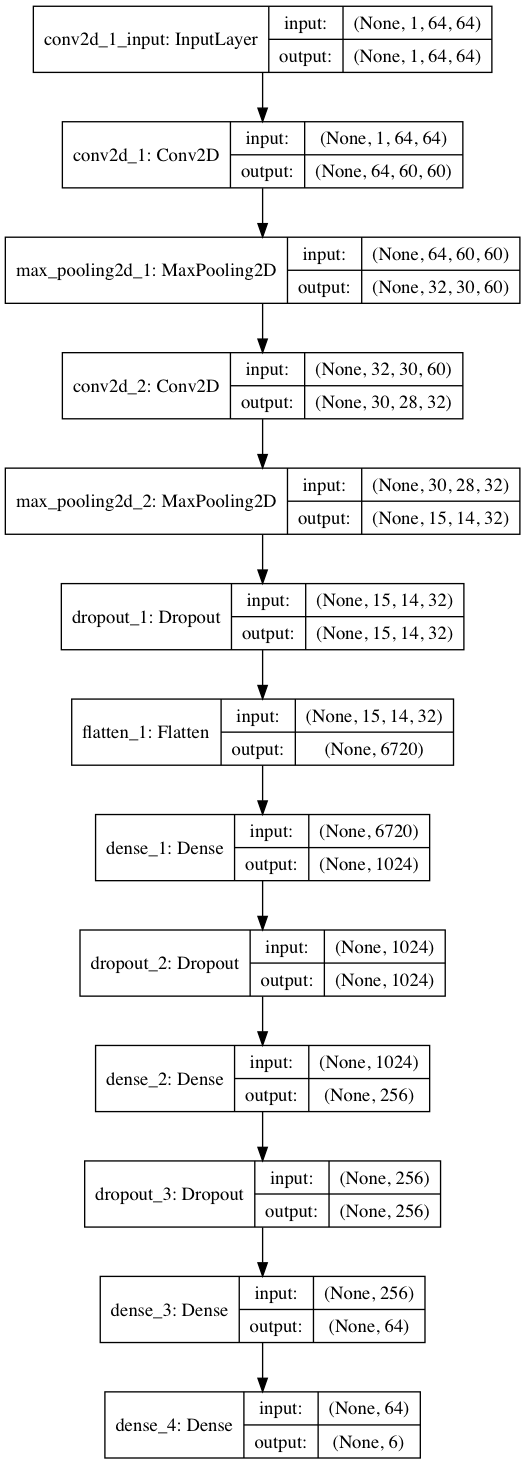
\includegraphics[scale=0.35]{pierwszy_plot}
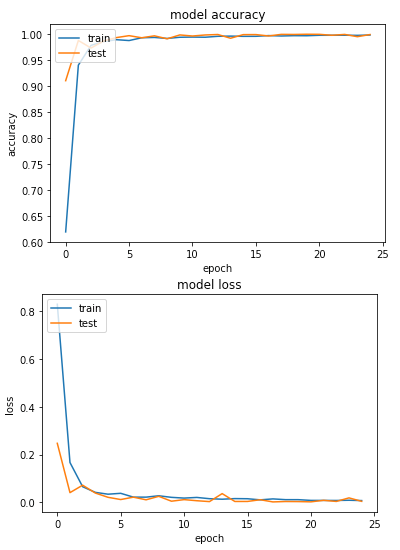
\includegraphics[scale=0.55]{pierwszy_accloss.png}

Rezulataty osiągnięte przez ten model były zdumiewające. Po pierwszej epoce
sieć uzyskała 61,98\% skuteczności ostatecznie osiągając wynik 99,88\% po 25 epokach.
Kolejne 10 epok praktycznie nie poprawiło już tego rezultatu.\\
Po analizie tego dokonania, okazało się że tak duża ilość zdjęć otrzymanych
z każdego ze zdjęć początkowych stworzyła zbiór w którym wiele zdjęć praktycznie się
powtarzało. Sieć nie miała żadnych problemów podczas testowania na zbiorze
do którego w teorii nie miała dostępu podczas treningu. Ten fakt spowodował konieczność
trenowania sieci na zbiorach zróżnicowanych pod kątem doboru różnych kolorów oraz
ilości zdjęć otrzymanych z jednego poczatkowego zdjęcia.

\paragraph{Model ze zróżnicowanymi zdjęciami} \mbox{}\\
Po stworzeniu modelu który wykazał, że zadanie stworzenia dobrze działającej sieci dla
tego problemu jest wykonalne, zabrano się do kolejnego etapu prac. W tym celu
wykorzystano zbiór złożony z 13 różnych zestawów kolorystycznych kości, oczek oraz tła,
liczący po 80640 i 20160 zdjęć na części treningową i testową.\\
W tym modelu wykorzystano architekturę nieznacznie zmienioną w stosunku pierwszego modelu.\\
Sieć uczona była przez 25, a następnie przez 10 epok.
Po pierwszych 25 epokach uzyskano dokladność 55,64\% co potwierdziło przypuszczenie
z przedniej sieci o możliwości pokrycia się zdjęć w zbiorach treningowym i testowym.
Kolejne 10 epok poprawiło wynik sieci do 65,30\%, pozwalając przy okazji zaobserwować
istotny fakt. W pierwszej sesji 25 epok, dokładność sieci przez ostatnie
5 epok oscylowała w okolicach 52\%. W drugiej sesji, niemalże od razu wartość
podniosła się do 56\%. Prawdopodobnie miało to związek ze sposobem w jaki dostarczane
są dane do modelu. Dane były ustalane losowo, ale dla każdej epoki w jednej sesji,
układ ten się nie zmieniał. Istniała szansa, że kiedy w następnej sesji zdjęcia
były przetwarzane w innej kolejności, umożliwiło to lepsze dopasowanie sieci i efekt
skoku jej dokładności.\\
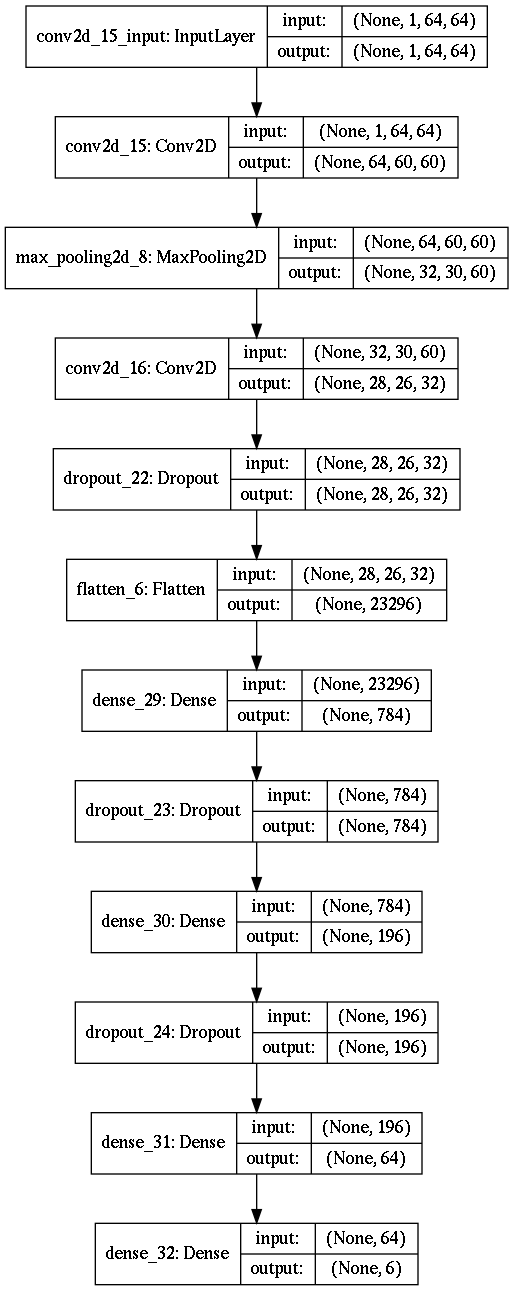
\includegraphics[scale=0.4]{modeladam_plot}
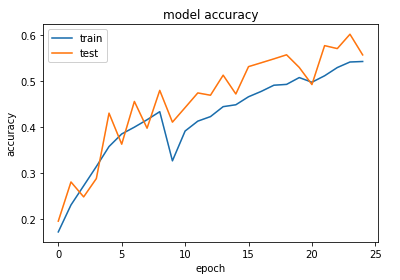
\includegraphics[scale=0.55]{adam_acc}

\paragraph{Model z wybranymi zdjęciami} \mbox{}\\
Znacząca różnica w dokładności między modelem z jednolitymi oraz zróżnicowanymi zdjęciami
doprowadziła do stworzenia sieci uczonej na zbiorze różnorodnych obrazów, ale
dobranymi tak, aby kontrast między tłem, a kością był wyraźny. Architektura sieci
jest identyczna jak w powyższych przykładach, jedyną różnicą jest przetwarzanie
wyselekcjonowanych obrazów. Zastosowanie 25 epok wystarczyło aby uzyskać dokładność
na poziomie 89,23\% co jest rezultatem zdecydowanie lepszym niż uzyskane wcześniej 55,64\%.\\
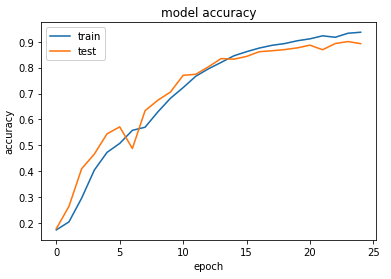
\includegraphics[scale=0.55]{adam_wybrane_acc}
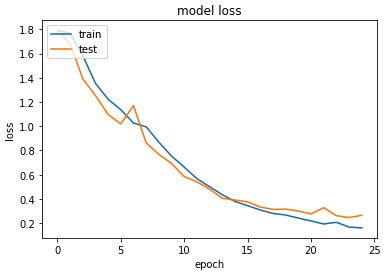
\includegraphics[scale=0.55]{adam_wybrane_loss}

\section{Analiza różnych optymalizatorów}
Jeżeli sama różnica w doborze konkretnych obrazów potrafi w tak dużym stopniu zmienić wyniki
otrzymane przez sieć, podjęto próbę przetestowania kilku z dostępnych w bibliotece Keras
optymalizatorów dla identycznych sieci oraz zbiorów danych. W tym celu postanowiono użyć
optymalizatorów RMSprop oraz SGD.\\
Oba modele z optymalizatorami RMSprop oraz SGD, zostały podobnie jak wcześniej opisany model
z optymalizatorem Adam poddane uczeniu przez 25 epok różnorodnych zbiorów obrazów. Wynik RMSprop
był zdecydowanie najlepszy i wyniósł 84,34\% skuteczności. Najgorszy rezultat w zestawieniu
uzyskał amodel korzystający z SGD, zdobywając jedynie 36,92\% poprawności. Pośrednim okazał
się Adam, który jak opisane wyżej, uzyskał 55,64\% po sesji uczenia przez 25 epok.\\
Wyniki te dowiodły, że optymalizator jest kluczowym parametrem \textit{(ang. hyperparameter)}
dla odpowiednio skutecznego uczenia. Uzyskany wynik dla RMSprop jest sporym zaskoczeniem,
ponieważ w licznych tekstach naukowych to Adam uznawany jest za jeden z najlepszych
optymalizatorów, ciesząc się ogromną popularnością. Również z tego powodu, pomimo
gorszego niż RMSprop wyniku, Adam będzie wykorzystywany w następnych modelach.\\
\textbf{Adam:}\\
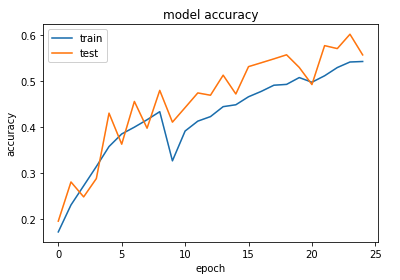
\includegraphics[scale=0.55]{adam_acc}
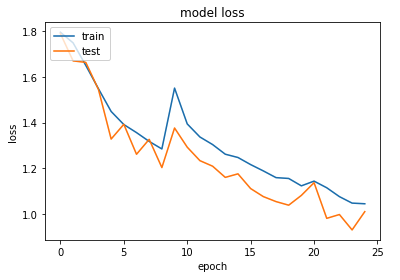
\includegraphics[scale=0.55]{adam_loss}\\
\textbf{RMSprop:}\\
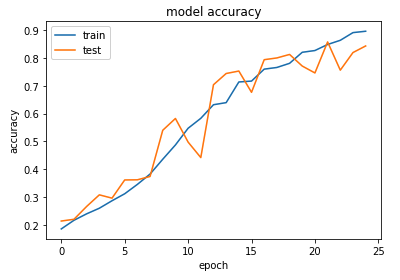
\includegraphics[scale=0.55]{rmsprop_acc}
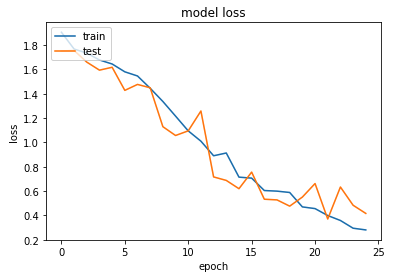
\includegraphics[scale=0.55]{rmsprop_loss}\\
\textbf{SGD:}\\
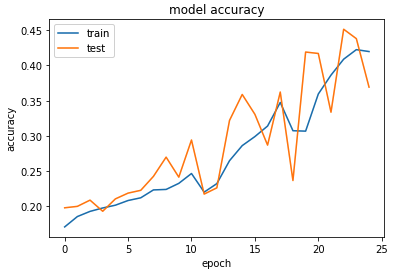
\includegraphics[scale=0.55]{sgd_acc}
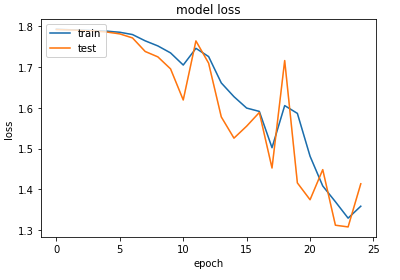
\includegraphics[scale=0.55]{sgd_loss}\\

\section{Wykorzystanie sieci AlexNet}
Sieć o nazwie AlexNet została zaprezentowana przez Alexa Krizhevskyego, Geoffreya Hintona oraz
Ilya Sutskevera w 2012 roku. Jej ideą jest zastosowanie większej ilośći warstw konwolucyjnych,
gdzie początkowe dwie warstwy mają filtry rozmiarów odpowiednio 11x11 oraz 5x5. Następnie
umieszczone są trzy warstwy konwolucyjne z filtrami 3x3, które w przeciwieństwie do pierwszych
dwóch warstw nie są rozdzielone warstwami z maxpoolingiem. AlexNet zdeklasowała rywali
w konkursie ILSVRC 2012 i swoimi rezultatami zszokowała wielu naukowców. Z racji tak świetnych
rekomendacji, zdecydowano się na realizację modelu przypominającego jej budowę.\\
Zastosowanie uproszczonej architektury, bazującej na idei sieci AlexNet pozwoliło
na osiągnięcie poprawności wynoszącej 98.88\% po 25 epokach. Na wykresie uczenia się
można zaobserwować, że przez pierwsze 10 epok prezycja przewidywań sieci w ogólnie nie
rosła. Obserwacja sugeruje, że sieci głębsze mogą potrzebować większej ilości epok
do rozpoczęcia procesu prawidłowego rozpoznawania obrazów.\\
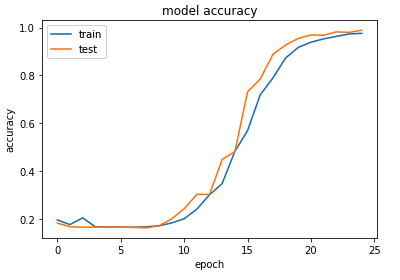
\includegraphics[scale=0.55]{alexnet_acc}
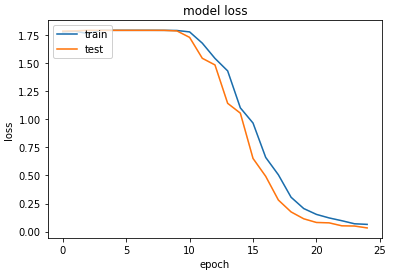
\includegraphics[scale=0.55]{alexnet_loss}

\section{Porównianie dla obrazów kolorowych i czarno-białych}
Obraz w skali szarości posiada jedynie jeden kanał odpowiadający jasności. Obrazy kolorowe RGB
posiadają trzy kanały informujące o nasyceniu odpowiednio czerwonego, zielonego i niebieskiego koloru.
Wzrost ilości informacji wiąże się z większym obciążeniem pamięci i większą ilością parametrów.
W celu weryfikacji różnicy między uczeniem obu rodzajów obrazów podjęto próbę porównania wyników
uczenia dla dwóch jednakowych sieci.\\
\textbf{Kolorowe RGB:}\\
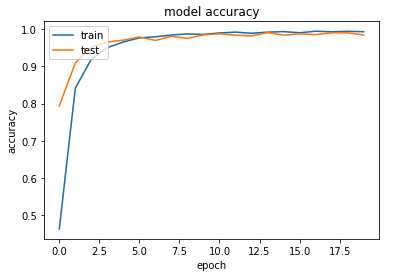
\includegraphics[scale=0.55]{comp_color_acc}
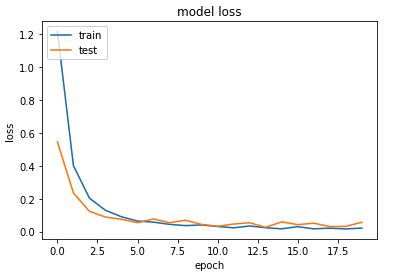
\includegraphics[scale=0.55]{comp_color_loss}\\
\textbf{Skala szarości:}\\
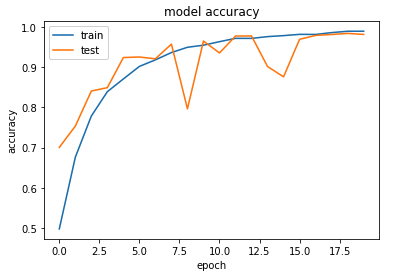
\includegraphics[scale=0.55]{comp_gray_acc}
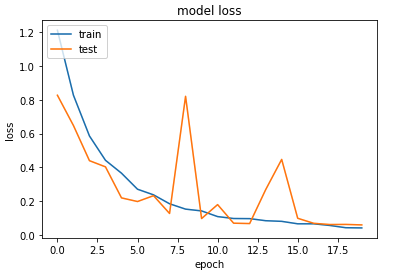
\includegraphics[scale=0.55]{comp_gray_loss}\\
Do tego eksperymentu wykorzystano narzędzie generatora dostępne w Keras, które umożliwia
przekazywanie obrazów do sieci bez konieczności wcześniejszego ładowania całego zbioru
do pamięci, umożliwiając pracę na bardzo dużych zestawach danych. Architektura obu
sieci była uproszczona, by zniwelować długi czas uczenia. Modele obu sieci znajdują się poniżej:\\\\
Oba modele po 20 epokach wykazały się bardzo zbliżonymi wynikami 98,47\% oraz 98,12\%
na korzyść sieci z kolorowymi obrazami. Lepiej radzący sobie model, dodatkowo nauczył
się bardzo szybko do poziomu 95\%, osiągając go już po 4 epoce, gdzie operujący na
obrazach w skali szarości osiągnął ten wynik po 10 epokach. Obserwacja ta może sugerować,
że większa różnica w wartościach dla kolorowych obrazów może przyśpieszać uczenie, ale
wymaga większej ilości pamięći i spowalnia każdą epokę o 15\%.

\section{Porównanie modelu sekwencyjnego i funkcyjnego biblioteki Keras}
\paragraph{Pierwsze użycie modelu funkcyjnego} \mbox{}\\
Standardowym sposobem na stworzenie sieci neuronowej w bibliotece Keras jest wykorzystanie
sekwencyjnego modelu, opierającego się na zasadzie umieszczania warstw na stosie. Bardziej
zaawansowaną możliwością jest wybranie modelu funkcyjnego API, który pozwala na budowę złożonych
sieci neuronowy m.in. z wieloma wyjściami, współdzielonymi warstwami i acyklicznymi grafami.\\
Zdecydowanie większe możliwości modelu funkcyjnego spowodowały chęć realizacji bardziej złożonych
sieci neuronowych. Pierwsza próba miała za zadanie odtworzyć sieć o identycznej budowie jak w
pierwszy model operujący na różnokolorowych zbiorach i porównać wyniki po uczeniu przez 25 epok.
Model został przedstawiony poniżej:\\
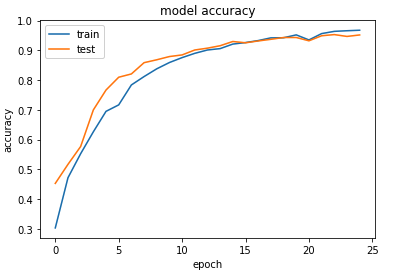
\includegraphics[scale=0.55]{adam_API_acc}
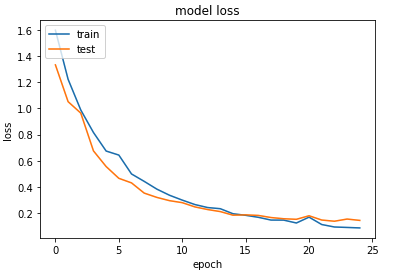
\includegraphics[scale=0.55]{adam_API_loss}\\
Zaskoczeniem była spora rozbieżność w ilości parametrów do nauczenia.W modelu sekwencyjnym
ich ilość wynosiła 18 milionów, a w modelu funkcyjnym API aż 25 milionów parametrów, co oznacza
40\% wzrost ich ilości oraz 50\% wzrost czasu potrzebnego na jedną epokę przy identycznie
zdefiniowanych warstwach. Ciężko uzasadnić tą różnicę, z grafu można wywnioskować, że
prawdopodobnie model ten inaczej uwzględniał filtry konwolucyjne, ponieważ rozmiar warstw
po ich zastosowaniu nie był jednakowy.\\
Niezależnie od tego, model osiagnął zdumiewająco dobry rezultat 95,17\% dokładności.
Wadą tego rozwiązania była, przez zwiększoną ilość parametrów i konieczność zastosowania
mniejszego rozmiaru partii obrazów jednocześnie dostarczanych sieci z powodów
problemów z pamięcią.

\paragraph{Pełne porównanie modeli} \mbox{}\\
Brak sugestii dostępnych w internecie oraz dokumentacji biblioteki Keras wyjaśniających różnice
w ilośc parametrów w modelach sekwencyjnym oraz API spowodował chęć stworzenia dwóch dużych,
identycznych modeli, bezpośrednio porównających ilość parametrów. Modele zostały jedynie
skompilowane w celu wyciągnięcia informacji o ich rozmiarach, ich uczenie zajęło by zbyt dużo czasu.\\
Po kompilacji, model sekwencyjny uzyskał 47 milionów parametrów, a model funkcyjny API
aż 500 milionów parametrów do nauczenia. Ta ogromna różnica spowodowała zaniechanie
kolejnych prac nad modelami funkcyjnymi z uwagi na wielokrotne zwiększenie czasu potrzebnego
na proces uczenia.

\section{Próby wykorzystania prostokątnych obrazów}
\paragraph{Doświadczenia zakończone niepowodzeniem} \mbox{}\\
Dotychczasowe modele korzystały ze zbiorów o obrazach w kształcie kwadratów z kośćmi
umieszczonymi w ich środkowej części. Drugi rodzaj przygotowanych zbiorów danych zwiększał
trudność zadania, dzięki zastosowaniu obrazów prostokątnych z mniejszym obszarem na
którym znajdowała się kostka w stosunku do pierwsze rodzaju obrazów.\\
Po uzyskaniu wielu bardzo dobrych wyników powyżej 90\% na obrazach o rozmiarach 64x64
przystapiono do prób znacznego zwiększenia obrazów prostokątnych.\\
Pierwszą próbą było wykorzystanie obrazów 320x240 zarówno w wersjach kolorowych jak
i w skali szarości. Jeden z modeli bazował na architekturze AlexNet, drugi bezpośrednio
ją kopiował, ale pomimo świetnego wyniku na mniejszych obrazach, w obu przypadkach
uczenie zakończyło się całkowitą klęską. Warto wspomnieć, że czas potrzebny na
jedną epokę był około 15-krotnie większy niż w przypadku obrazów 64x64.\\
Ostania próba z obrazami w tym rozmiarze, zakładała użycie uproszczonej architektury
podobnie jak przy porównaniu uczenia obrazów RGB i w skali szarości. Finalnie, tak jak
wcześniej, pomimo 20 epok sieć nie wykazała żadnego postępu w rozpoznawaniu kości.\\\\
Niepowodzenia spowodowały konieczność zmniejszenia zbiorów przez ograniczenie rozmiarów obrazów.
Problemem podczas zmniejszania była chęć uniknięcia problemów z brakiem ostrości
oczek na kostce co mogłoby uniemożliwić skuteczną naukę. Zdecydowano się na dwukrotne
zmniejszenie rozmiarów obrazów, licząc że pozwoli to na zaobserwowanie chociaż niewielkich
postępów.\\
Sieć bazująca na zdjęciach 160x120 była pierwszą próbą, gdzie zamiast jak dotychczas
kwadratowych, użyto prostokątnych filtrów konwolucyjnych. Proces uczenia po 20 epokach
niestety również zakończył się niepowodzeniem.\\
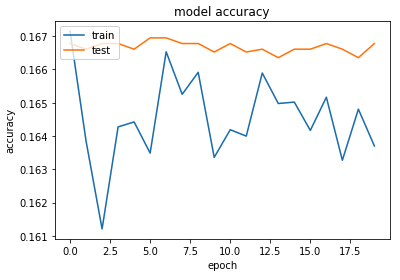
\includegraphics[scale=0.55]{not_learned_acc}
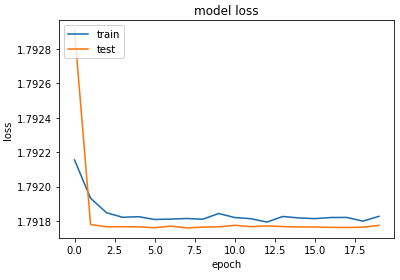
\includegraphics[scale=0.55]{not_learned_loss}

\paragraph{Wytrenowany prostokątny model} \mbox{}\\
Powyższe porażki oraz wcześniejsze sukcesy na kwadratowych obrazach sugerowały, że
prawdopodobnie modele nie są błedne, jedynie obrazy mogą mieć za duży rozmiar. Ta hipoteza
rozpoczeła proces dobierania odpowiedniej rozdzielczości zdjęć tak by były małe, jednocześnie
unikając rozmycia oczek na kostce nie. Najlepszym wyborem okazały się zdjęcia w rozmiarze 106x79,
zachowujące proporcje jak obrazy 160x120, ale posiadające o 50\% mniejszą liczbę parametrów.\\
Pierwsza próba przeprowadzona przez 20 epok z filtrami konwolucjnymi o prostokątnych
kształtach wreszcie zakończyła się sukcesem. Sieć osiągnęła wynik 68,03\% co nie
było świetnym rezultatem, ale dawało informację, że dalsza nauka jest możliwa.\\
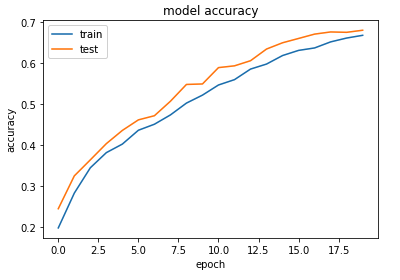
\includegraphics[scale=0.55]{rect_acc}
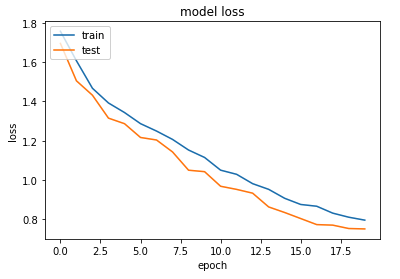
\includegraphics[scale=0.55]{rect_loss}

\section{Doskonalenie modelu z prostokątnymi obrazami}
Po pierwszym sukcesie sieci z obrazami prostokatnymi, podjęto decyzję o jej ulepszeniu.
Zaczęto od próby zmniejszenia ilości parametrów przez zamianę większych filtrów konwolucyjnych,
większą ilością mniejszych, co znacząco zmniejszało ilość parametrów sieci potrzebną do nauczenia
\textit{Substituting Big convolution} \cite{substBigConv}.
Po zaaplikowaniu ulepszeń i nauce sieci, okazało się że sieć nie poprawiła się w żadnym
stopniu. Prawodopodobnym powodem była zmiana architektury sieci wraz z powtórnym
zastosowaniem kwadratowych filtrów.\\\\
Drugim pomysłem na ulepszenie sieci było zastosowanie zastępowania większych filtrów
kilkoma mniejszymi połączonego ze zamianą funkcji aktywacji ReLU na LeakyReLU w celu uniknięcia
możliwych do wystąpienia problemów z zanikającym neuronem. Ulepszenie jednak podobnie
jak wcześniejsze nie sprawdziło się w ogóle i nie umożliwiło poprawy dokładności sieci.

\section{Najskuteczniejszy model z prostokątnymi obrazami}
Wykres procesu uczenia sieci z obrazami 106x79 kształtem przypominał funkcję logarytmiczną
co nasuneło pomysł ze zwiększeniem ilości epok. Podjęto decyzję o kontynuacji uczenia
do kolejno 40, 60, 80 i 100 epok.\\
Podejście to okazało się bardzo skuteczne, ponieważ po każdych 20 epokach
sieć odnosiła lepsze rezultaty, które prezentowały się nastepująco:\\
20 epok: 68,03\%\\
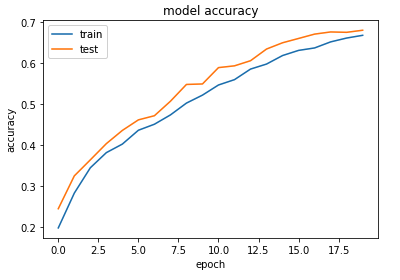
\includegraphics[scale=0.55]{rect_acc}
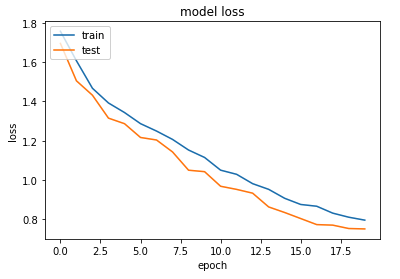
\includegraphics[scale=0.55]{rect_loss}\\
40 epok: 78,21\%\\
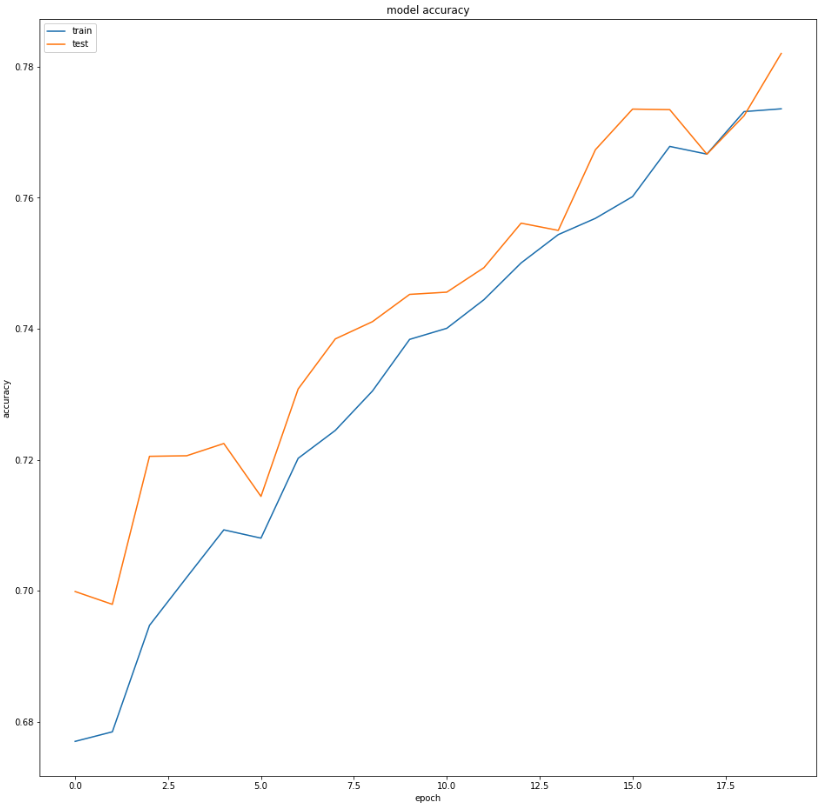
\includegraphics[scale=0.265]{rect_20-40_acc}
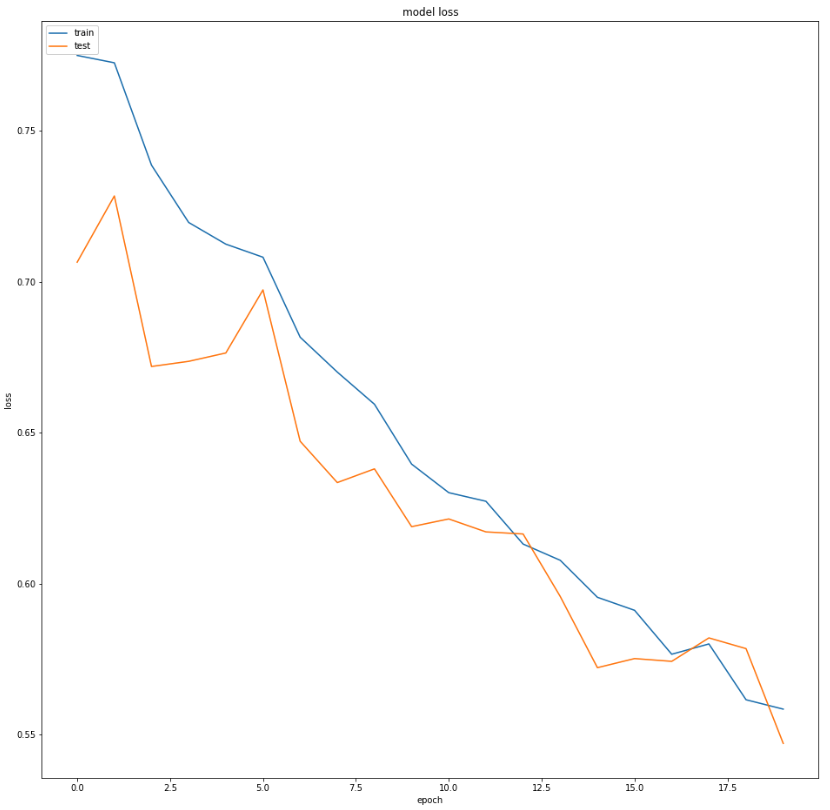
\includegraphics[scale=0.265]{rect_20-40_loss}\\
60 epok: 81,59\%\\
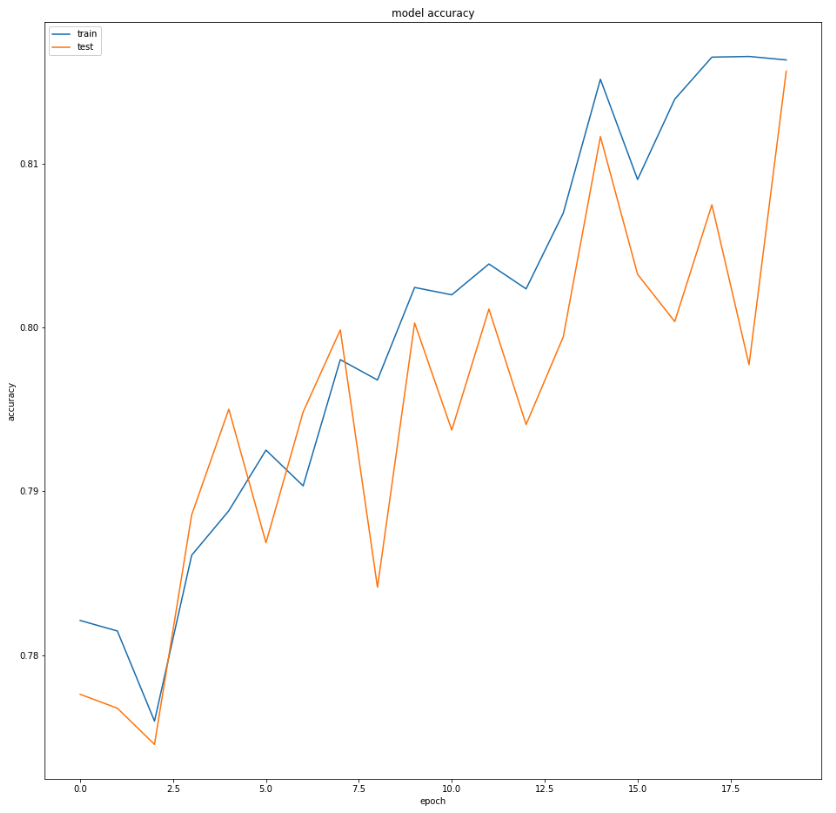
\includegraphics[scale=0.265]{rect_40-60_acc}
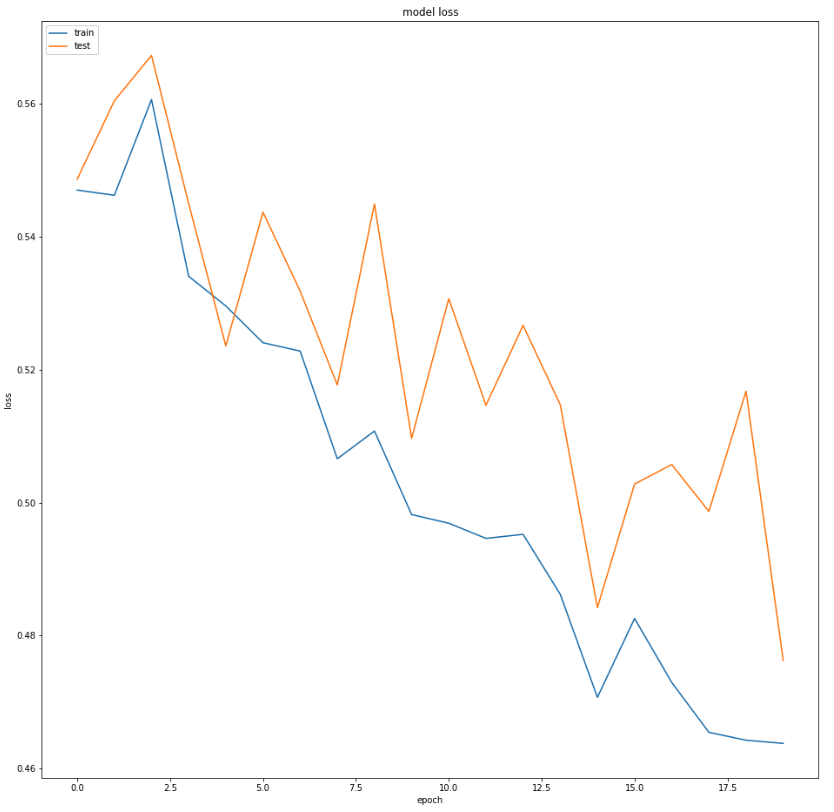
\includegraphics[scale=0.265]{rect_40-60_loss}\\
80 epok: 82,39\%\\
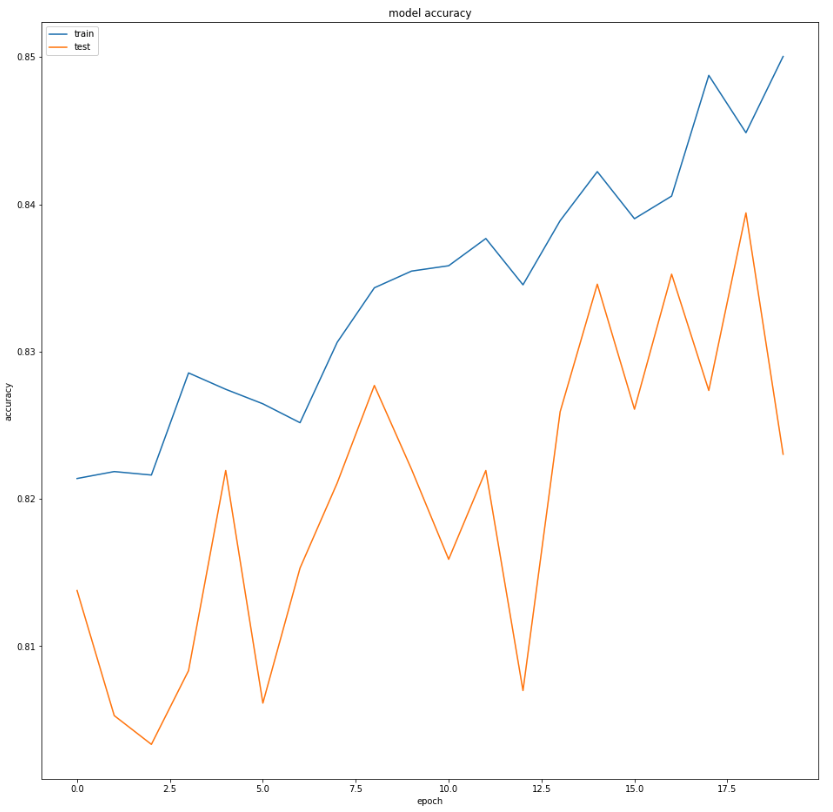
\includegraphics[scale=0.265]{rect_60-80_acc}
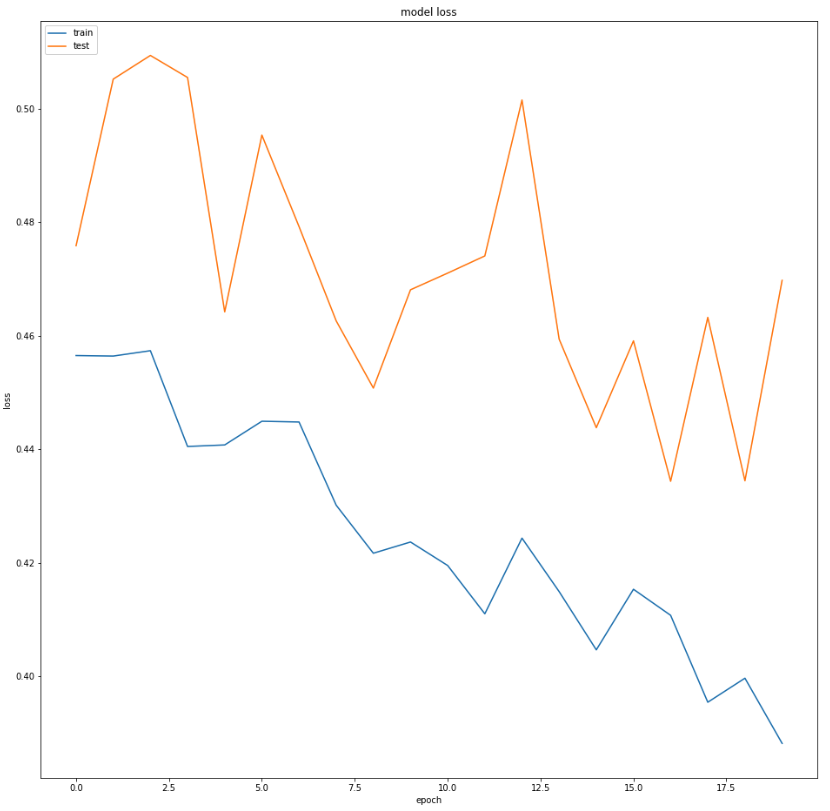
\includegraphics[scale=0.265]{rect_60-80_loss}\\
100 epok: 84,67\%\\
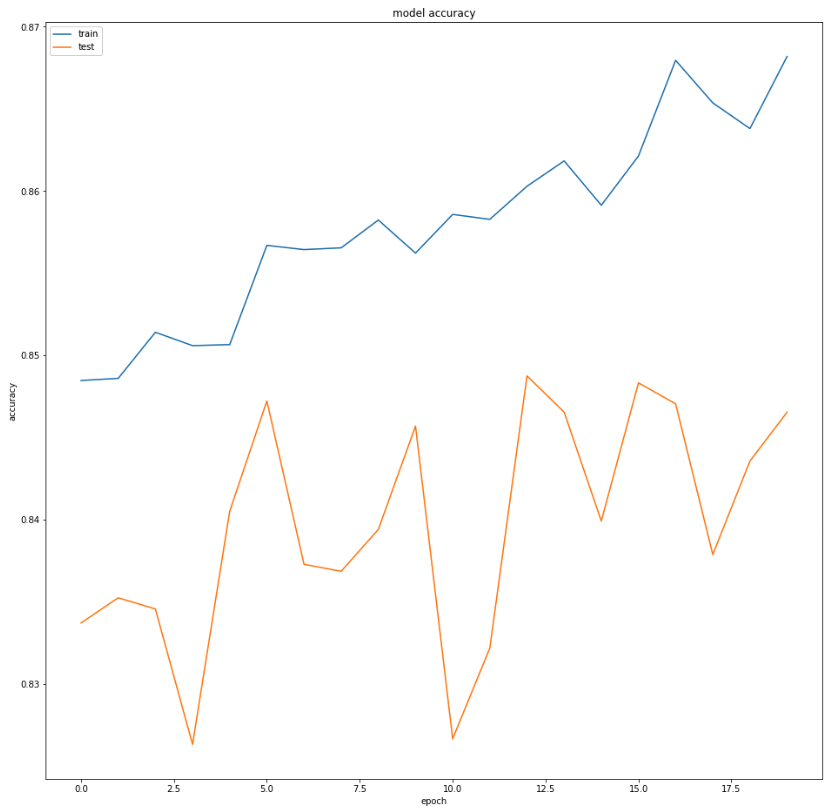
\includegraphics[scale=0.265]{rect_80-100_acc}
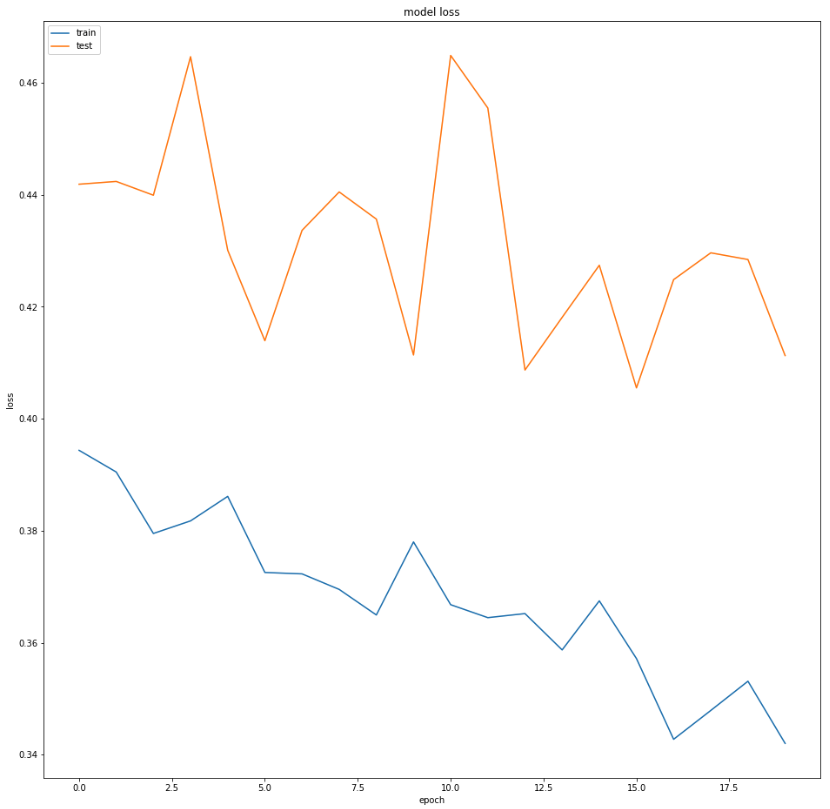
\includegraphics[scale=0.265]{rect_80-100_loss}\\
Wyniki uświadamiają, że prawdopodobnie nawet nieudane próby z większymi zdjęciami
mogłyby się powieść, konieczne byłoby jedynie zwiększenie ilości epok. Wiąże się to jednak
z ogromnym nakładem czasu, ponieważ prawdopodobnie sensowne rezultaty można by osiągnąć
dopiero po 100 epokach.
